\documentclass{ltjsarticle}
\usepackage{amsmath}
\usepackage{amssymb}
\usepackage{ascmac}
\usepackage[dvipdfmx]{graphicx}
\usepackage{tabularx}
\usepackage[colorlinks=true, allcolors=blue]{hyperref}
\usepackage{fancybox}
\usepackage{tikz}
\usepackage{subcaption}
\usetikzlibrary{shapes,arrows}

\begin{document}

\title{100. 深層学習 day4}
\author{秋葉洋哉}
\maketitle

\section{強化学習}
\subsection{概要}

強化学習は、エージェントが環境と相互作用し、環境から報酬を受け取ることで、最適な行動を学習する手法である。強化学習の特徴は、報酬を最大化するような行動を学習することである。ただし、報酬を得るためにはどうしたらよいか、という問題は、非自明である場合が多く、報酬のみではスパースで扱いづらいため、途中の過程で出てくる状態や、エージェントの行動に価値を付与し、その価値を最大化させる問題に置き換えて考える。よって、強化学習では、状態、行動、報酬、方策、価値関数の5つの要素で構成される。
\begin{table}[ht]
  \centering
  \begin{tabularx}{\textwidth}{|X|X|X|X|}
  \hline
  要素 & 変数 & 定義 & (例)将棋の場合 \\ \hline \hline
  状態 & s(state) & エージェントが環境と相互作用する際の状態 & 将棋盤の状態 \\ \hline
  行動 & a(action) & エージェントが環境に対して取る行動 & 駒を動かす \\ \hline
  報酬 & r(reward) & エージェントが環境から受け取る報酬 & 勝敗 \\ \hline
  方策 & $\pi$(policy) & エージェントが状態に対して取る行動を決定するための戦略 & 次の一手 \\ \hline
  価値関数 & V(Value), Q(Quality) & エージェントが状態や行動に対してどれだけ価値があるかを表す関数 & 評価値 \\ \hline
  \end{tabularx}
  \caption{強化学習で用いられる単語の定義と例}
  \label{tab:reinforcement_learning}
\end{table}
\par
強化学習の手法には、方策勾配法、Q学習、SARSA、DQN、DDPG、PPOなどがある。
主に3つの方針が用いられる。
\begin{enumerate}
  \item 方策ベース : 状態価値$V$を推測し、以降の状態価値の現在割引和(同じ報酬が得られるなら早い方がいいという考え方)を最大化するような方策$\pi$を学習する
  \item 価値ベース : エージェントの行動価値$Q$を推測し、以降の行動価値の現在割引和を最大化するような方策$\pi$を学習する
  \item モデルベース : 環境が分かっているという仮定のもと、価値最大化をプランニングする
\end{enumerate}

\par
以下に、強化学習システムの画像を示す。
\begin{figure}[htbp]
  \centering
  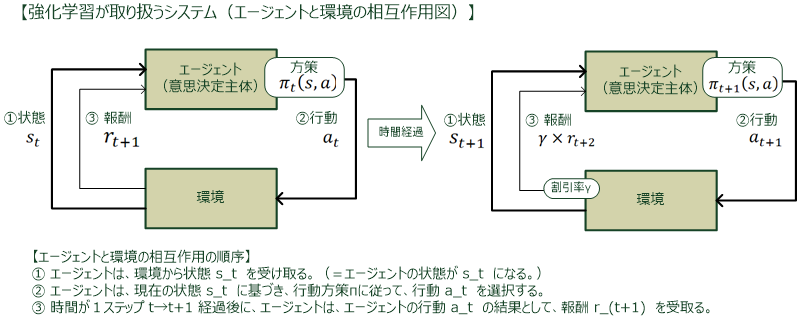
\includegraphics[width=15cm]{./capture/reinforcement_learning.png}
  \caption{強化学習システムの概要}
  \label{reinforcement_learning}
\end{figure}

\par
ここで重要な点は、環境について事前に完璧な知識があれば最適な行動を決定することができるが、環境についての知識が不完全である場合最適な行動を学習することが困難であるということである。
強化学習の場合、不完全な知識を元に行動しながら、データを収集することで最適な行動を学習していく。
\par
強化学習は、価値関数をどのように設定するか、そして、その価値関数を最大にするにはどのような方策関数が必要かという問題を解くことが目的となる。



\subsection{簡単な歴史}
\begin{table}[ht]
  \centering
  \begin{tabular}{|c|p{10cm}|}
  \hline
  年 & 説明 \\
  \hline
  1950年代 & 強化学習の始まり。Richard Bellmanが動的計画法を提案。 \\
  1960年代 & Richard SuttonがTD学習を提案。 \\
  1989年 & Christopher WatkinsがQ学習を提案。 \\
  1992年 & Gerald TesauroがバックギャモンのAIを開発。 \\
  2006年 & Geoffrey Hintonが深層強化学習を提案。 \\
  2013年 & DeepMindがDQNを提案し、Atari 2600のゲームで人間を超える性能を達成。 \\
  2016年 & AlphaGoが囲碁の世界チャンピオンを破り、強化学習の可能性を示す。 \\
  \hline
  \end{tabular}
  \caption{強化学習の歴史}
  \label{tab:comparison}
\end{table}
\par
かつて、強化学習はテーブルベースの手法が主流だった。その手法とは、状態と行動の組み合わせに対して価値を表すテーブルを用意し、そのテーブルを更新することで最適な行動を学習する手法である。しかし、テーブルベースの手法は状態や行動の数が増えるとテーブルのサイズが指数関数的に増加するため、現実の問題には適用しづらいという問題があった。
\par
その後、そのテーブルの対応付けを関数で表現することで、状態や行動の数が増えても対応できる手法が提案された。この手法が、ディープラーニングを用いた強化学習である。ディープラーニングを用いた強化学習は、状態や行動の数が増えても対応できるため、現実の問題に適用できるようになり、強化学習が注目されるようになった。

\subsection{価値関数}
価値関数には状態価値関数と行動価値関数の2つがある。近年の強化学習では、行動価値関数を用いることが一般的である。
\begin{enumerate}
  \item 状態価値関数$V(s)$:状態$s$において得られる報酬の期待値 (状態のみを入力とする関数)
  \item 行動価値関数$Q(s,a)$:状態$s$において、行動$a$を取った後に得られる報酬の期待値 (状態と行動を入力とする関数)
\end{enumerate}

\subsection{方策関数}
方策関数$\pi$は、状態$s$において行動$a$を取る確率を表す関数である。
方策関数の目的は、価値関数を最大にするような行動を決定することである。
例えば、将棋の場合は、価値関数が評価値の値を決定し、方策関数が次の手を決定する。

\subsection{最適化問題の解き方}
強化学習における最適問題の解き方は、主に以下の3つの方法がある。
\begin{enumerate}
  \item 動的計画法 :  選択肢を一つずつ増やしていき、逐次的に最適解を求めていく方法
  \item モンテカルロ法 : 方策ベースの手法で用いられ、ロールアウトによって疑似的にいくつかの選択肢を比較し、方策を決定する方法
  \item TD法 : 価値ベースの手法で用いられ、tステップ後の行動価値までを考えたうえでの行動選択の最適化を行う方法
\end{enumerate}

\subsubsection{方策勾配法}
方策勾配法は、方策関数を直接更新する手法である。方策勾配法は、方策関数の勾配を求め、その勾配の方向に方策関数を更新することで、最適な方策関数を学習する。
方策勾配法では、方策の勾配$\theta$を更新していく。
\begin{align}
  \theta^{(t+1)} = \theta^{(t)} + \epsilon \nabla J(\theta)
\end{align}
ここで、$J(\theta)$は方策関数の期待報酬であり、$\epsilon$は学習率である。
この式では、期待報酬$J(\theta)$を、方策関数の期待報酬を最大化するように更新していく。
第二項は、方策関数の勾配を求めるための式であり、以下のように表される。
\begin{align}
  \nabla_{\theta} J(\theta) &= \nabla_{\theta} \sum_{a\in A} \pi_{\theta}(a | s) Q^{\pi}(s, a) \\
  &= \mathbb{E}_{\pi_{\theta}}[\nabla_{\theta} \log \pi_{\theta}(a | s)Q^{\pi_{\theta}}(s, a)]
\end{align}
ここで、$\pi_{\theta}$は方策関数、$Q^{\pi_{\theta}}(s, a)$は行動価値関数である。
下付きの$\theta$や、$\pi_{\theta}$は、方策関数のパラメータであることを表している。

\clearpage

\section{AlphaGo}
\subsection{AlphaGo Lee}
\subsubsection{概要}
AlphaGo Leeは、2016年にGoogle DeepMindが開発した囲碁のAIである。19×19×48の囲碁の盤面を入力すると、次の一手・評価値を出力する。各目毎の48チャンネルは、表\ref{tab:AlphaGo_Lee}以下の通りである。
Policy Netでは、19×19のすべての目の着手確率、Value Netでは、評価値を出力する。

\begin{table}
  \centering
  \begin{tabular}{lll}
    \hline
    内容 & チャンネル数 & 説明 \\
    \hline
    石の色 & 3 & 自分の石、相手の石、空き目 \\
    オール1 & 1 & すべての要素が1である盤面 (1チャンネルすべてが1である盤面) \\
    着手履歴 & 8 & 過去8手の着手 (チャンネル1つに1つの石が対応) \\
    呼吸点 & 8 & 該当の位置に石がある場合、その石を含む連の呼吸点の数 \\
    取れる石の数 & 8 & 該当の位置に石を打った場合、取れる石の数 \\
    取られる石の数 & 8 & 該当の位置に石を打たれた場合、取られる石の数 \\
    着手後の呼吸点の数 & 8 & 該当の位置に石を打った場合、その石を含む連の呼吸点の数 \\
    着手後にシチョウで取れるか & 1 & 該当の位置に石を打った場合、シチョウで隣接連を取れるかどうか \\
    着手後にシチョウで取られるか & 1 & 該当の位置に石を打った場合、シチョウで隣接連を取られるかどうか \\
    合法手 & 1 & ルールに見合った手であるかどうか \\
    オール0 & 1 & すべての要素が0であるかどうか \\
    手番 & 1 & 現在の手番が黒番であるかどうか(ValueNetのみ) \\
    \hline
  \end{tabular}
  \caption{AlphaGo Leeの入力データ}
  \label{tab:AlphaGo_Lee}
\end{table}

\begin{figure}[htbp]
  \centering
  \begin{subfigure}[b]{0.45\textwidth}
    \centering
    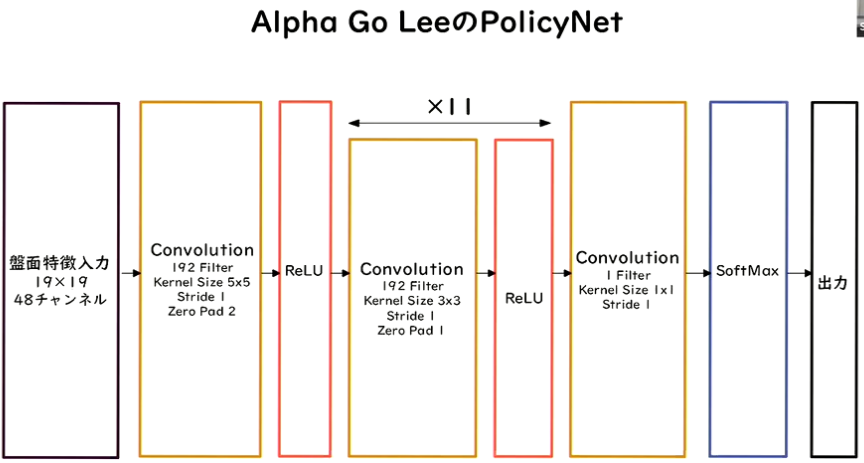
\includegraphics[width=\textwidth]{./capture/AlphaGo_Lee_PolicyNet.png}
    \caption{方策関数: Policy Net}
    \label{fig:Swish}
  \end{subfigure}
  \hfill
  \begin{subfigure}[b]{0.45\textwidth}
    \centering
    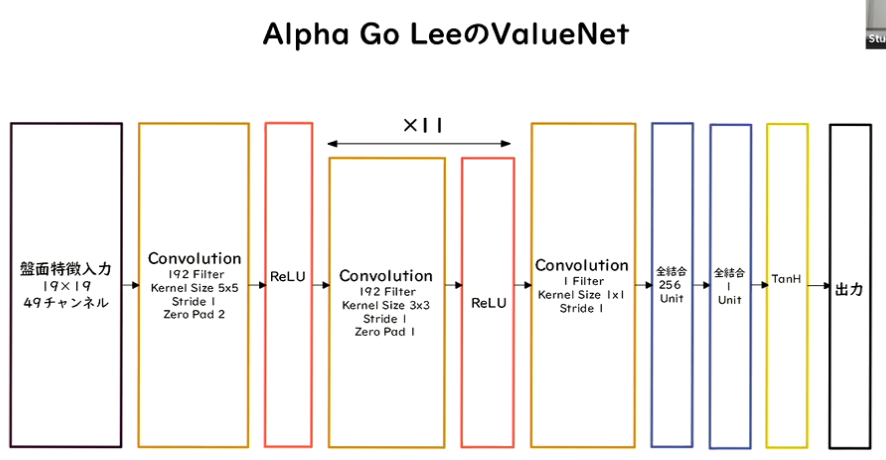
\includegraphics[width=\textwidth]{./capture/AlphaGo_Lee_ValueNet.png}
    \caption{価値関数: Value Net}
    \label{fig:LeakyReLU}
  \end{subfigure}
  \caption{AlphaGo Leeで用いられる方策関数と価値関数}
\end{figure}

\subsubsection{AlphaGo Leeの学習}
AlphaGoの学習は以下のステップで行われる。
\begin{enumerate}
  \item 教師あり学習によるRollOut PolicyとPolicy Netの学習
  \item 強化学習によるPolicy Netの学習
  \item 強化学習によるValue Netの学習
\end{enumerate}
以下では、それぞれのステップについて説明する。
\par
RollOut Policyとは、ニューラルネットワークではなく、線形の方策関数で、高速に着手確率を出すために用いられる。強化学習ではPolicy Netの学習1回に対して3ミリ秒、計$10^8$オーダーの学習回数が必要となるため、1手打つのに莫大な時間がかかる。そのため、RollOut Policyを用いて、アバウトだが高速に着手確率を出す($1マイクロ秒$/1学習)ことで、後々のPolicy Netの学習を効率化する。
RollOut Policyは、教師あり学習によって学習される。教師データは、人間の棋譜が用いられる。 
また、Policy Netも同様に人間の棋譜を用いて教師あり学習によって学習する。
\par
PolicyNetは、いわばBotであり、自分自身が最も身近な対戦相手となるため、PolicyNet同士で対戦させることで、PolicyNetの学習を行うのが効率的である。しかし、現状のPolicyNet同士で対戦させると、PolicyNet同士が同じような戦略を取るため、過学習が発生しやすい。
\par
そこで、PolicyNetの学習にはPolicyPoolと呼ばれる複数のPolicyNetの集合を用いる。
PolicyPoolは、PolicyNetの学習過程を500Iteration毎に保存したものである。PolicyPoolからPolicyNetをランダムに選択したモデルと、現状のPolicyNetを対戦させ、その結果を用いて方策勾配法で学習を行う。
こうすることで、PolicyNet同士が同じような戦略を取ることを防ぎ、過学習を防ぐことができる。

\subsubsection{強化学習によるValue Netの学習}
ValueNetでは、PolicyNetの学習時の対局結果を教師データとして、教師あり学習を行う。
以下に教師データの作成手順を示す。
\begin{enumerate}
  \item まず、教師あり学習で作成したPolicyNet (SL PolicyNet)で$N$手までを打つ。
  \item その後、$N+1$手目の手をランダムに選択し、その手で進めた局面を$S(N+1)$とする。
  \item $S(N+1)$から強化学習で作成したPolicyNet (RL PolicyNet)で終局まで打ち、その結果の報酬を$R$とする。
  \item $S(N+1)$と$R$を教師データ対としてValueNetの入力とし、平均二乗誤差を最小化するように学習を行う。
\end{enumerate}

\par
AlphaGoにおける強化学習の学習手法として、モンテカルロ木探索という手法が最も有効とされている。

\subsubsection{モンテカルロ木探索}
モンテカルロ木探索は、盤面の価値や勝率予測値を考えずに、現局面から末端局面までランダムにシュミレーション(PlayOutと呼ぶ)を行い、その勝敗を集計して着手の優劣を決定する手法である。
\par
モンテカルロ木探索は、ある手を選んだ場合のシュミレーション回数が一定数を超えた時にその手を開始とする局面からの計算を打ち切り、その手を着手した後の局面をシュミレーション開始局面として、再度シュミレーションを行って、探索木を成長させていく。

\subsection{AlphaGo Zero}
\subsubsection{概要}
AlphaGo Zeroは、2017年にGoogle DeepMindが開発した囲碁のAIである。AlphaGo Zeroは、AlphaGo Leeと比較して以下の点が改善されている。
\begin{enumerate}
  \item 教師あり学習を一切行わず、強化学習のみで作成
  \item 特徴入力からヒューリスティックな要素(表\ref{tab:AlphaGo_Lee})を排除し、石の配置のみを入力とした
  \item PolicyNetとValueNetの統合
  \item Residual Networkを導入
  \item モンテカルロ木探索からRollOut Policyを排除
\end{enumerate}
\begin{figure}[htbp]
  \centering
  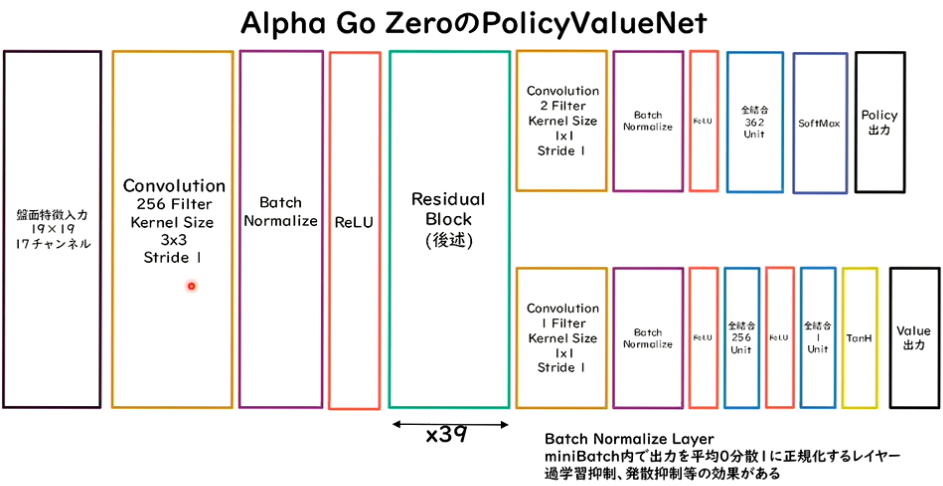
\includegraphics[width=15cm]{./capture/AlphaGo_Zero_PolicyValueNet.png}
  \caption{AlphaGo Zeroの方策価値関数 : Residual Networkの後にネットワークが2つに分岐していることが特徴である。}
  \label{fig:AlphaGo_Zero}
\end{figure}

\subsubsection{Residual Network}
Residual Networkとは、勾配消失問題を解決するために提案されたニューラルネットワークの構造である。
Residual NetworkはResidual Blockと呼ばれる単位を重ね合わせた (AlphaGo Zeroの場合は39層) ネットワークである。Residual Blockの中では入力に対して畳み込み・プーリング・活性化関数を適用した結果を、元の入力と足し合わせる。
このショートカット結合は、いわばそのBlock内の畳み込み層をドロップアウトさせているものだと考えることができる。ドロップアウトではランダムにノードを削除するが、Residual Networkでは、層を残したまま、その層の重みを0にすることで無効化する。つまり、スルーする層を学習するドロップアウトと考えることができる。
Residual Networkは、深いネットワークに対して勾配消失問題を解決するだけでなく、学習の収束を早める効果がある。

\subsubsection{AlphaGo ZeroにおけるNetworkの工夫}
AlphaGo Zeroでは、以下の工夫が施されている。
\begin{enumerate}
  \item Residual Blockに対してBottleneckの導入 (1x1畳み込みを用いて次元削減)
  \item Residual Blockに対してPreActivationの導入 (Batch Normalizationと活性化関数の順序を入れ替える)
  \item Network構造に対してWideResNetの導入 (フィルター数をk倍に増やし、GPUを効率的に用いる)
  \item WideResNetに対してPyramidNetの置き換え (各層でFilter数を増やす)
\end{enumerate}

\clearpage
\section{軽量化・高速技術}
\subsection{分散深層学習}
深層学習は多くのデータを使用したり、パラメータ調整のための計算量が多いため、複数の計算資源(ワーカー)を使用して、並列的にニューラルネットを構成することで、効率の良い学習を行うことが必要である。
そのために行われる高速化は大きく分けて
\begin{enumerate}
  \item データ並列化 (図\ref{fig:parallelism}左)
  \item モデル並列化 (図\ref{fig:parallelism}右)
  \item GPUによる高速化
\end{enumerate}
がある。
ちなみに、機械学習モデルの計算量は10倍/年の割合で増加している。一方で、GPUの性能は2倍/年の割合で増加しているため、GPUの性能を最大限に引き出すことが重要である。

\begin{figure}[htbp]
  \centering
  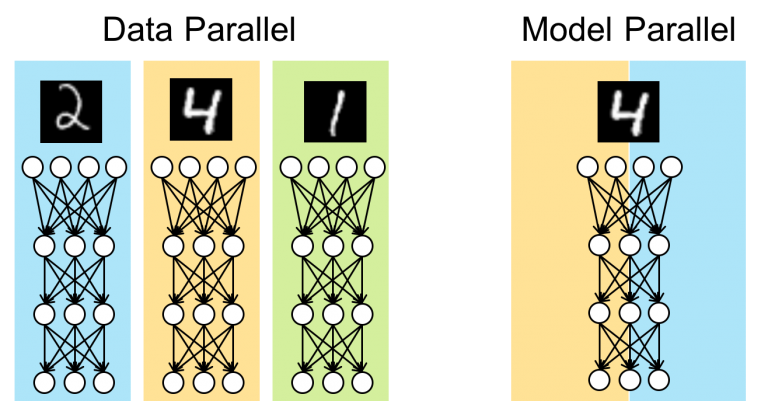
\includegraphics[width=15cm]{./capture/parallelism.png}
  \caption{データ並列化とモデル並列化のイメージ図(https://tech.preferred.jp/ja/blog/model-parallelism-in-dnn より引用)}
  \label{fig:parallelism}
\end{figure}

\subsubsection{データ並列化}
データ並列化は、元のビッグデータを複数の計算機で分割して学習させる方法で、同期型と非同期型の2つの手法がある。
\par
同期型は、親モデルとなる1つのモデルを複数のワーカーに分配し、それぞれのワーカーで学習を行い、各ワーカーで学習した時の誤差の勾配を平均化して、親のモデルに反映し、パラメータが更新する手法である。そうして、更新されたモデルを再度ワーカーに分配して学習を進める。
同期型は、各ワーカーが計算が終わるのを待ち、全ワーカーの勾配が出たところで勾配の平均を計算し、親モデルのパラメータを更新する。
\par
非同期型は、各ワーカーが独立して学習を行い、出来上がったモデルをパラメータサーバーに送り(push)、送った後、ワーカーはパラメータサーバーにあるモデルを取得(pop)して新しく学習を始める。パラメータサーバーは、先入れ先出しのキューであるため、ワーカーが送ったモデルが順番に処理される。
\par
同期型は、全ワーカーの計算が終わるのを待つため、計算時間がかかるが、パラメータの更新が安定している。一方、非同期型は、ワーカーが独立して学習を行うため、計算時間が短いが、パラメータの更新が不安定である。
例えば、世界中のスマートフォンを使って、分散深層学習を行う場合、非同期型が適しているが、GPUを使って分散深層学習を行う場合、同期型が適している。

\subsubsection{モデル並列化}
モデル並列化は、親モデルとなる1つのモデルを複数のワーカーに分配し、それぞれのワーカーでモデルの一部分を学習させる方法である。モデルの分割方法は、層ごとに分割する方法や、分岐した部分を分割する方法がある。
モデル並列化は1台の計算機内でGPUを用いて学習を行わせる場合が多く、モデルのパラメータ数が多いほどスピードアップの効率も向上する。

\subsubsection{GPUによる高速化}
GPU(図\ref{fig:GPU})は、CPU(図\ref{fig:CPU})に比べて大量のデータを並列処理することが得意である。そのため、深層学習の学習にはGPUを用いることが一般的である。もともとは、グラフィック描画のために開発されたGPUであるが、その並列処理能力を活かして、深層学習の学習に用いられるようになり、そうしたグラフィック用途以外の用途で用いられるGPUをGPGPU (General-Purpose computing on Graphics Processing Units)と呼ぶ。
\par
CUDA (Compute Unified Device Architecture)は、NVIDIAが提供するGPU向けの開発環境である。CUDAを用いることで、GPUを用いた高速な計算が可能となる。
OpenCLは、Appleが提唱したGPU向けのプログラミング環境である。OpenCLは、NVIDIAのCUDAと比較して、ハードウェアに依存しないため、様々なハードウェアで利用することができる。
\par
TensorflowやPyTorchを用いる場合、ユーザーはCUDAやOpenCLを意識することなく、GPUを用いた高速な計算を行うことができる。
\begin{figure}[htbp]
  \centering
  \begin{subfigure}[b]{0.45\textwidth}
    \centering
    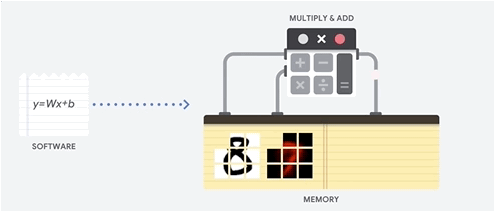
\includegraphics[width=\textwidth]{./capture/CPU.png}
    \caption{CPU}
    \label{fig:CPU}
  \end{subfigure}
  \hfill
  \begin{subfigure}[b]{0.45\textwidth}
    \centering
    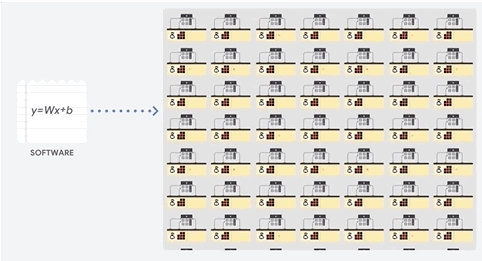
\includegraphics[width=\textwidth]{./capture/GPU.png}
    \caption{GPU}
    \label{fig:GPU}
  \end{subfigure}
  \caption{CPUとGPUの比較 : CPUは計算を行った結果をメモリに書き込む。GPUは算術論理演算装置(ALU)を2500$\sim$5000個搭載し、数千の乗算と加算を行う。(https://cloud.google.com/tpu/docs/intro-to-tpu?hl=ja より引用)}
\end{figure}


\subsubsection{TPUによる高速化}
TPU (Tensor Processing Unit) (図\ref{fig:TPU})は、Googleが開発したAI向けのASIC (Application-Specific Integrated Circuit)である。TPUは、GPUに比べて、深層学習の学習に特化しており、高速な計算が可能である。
\begin{figure}[htbp]
  \centering
  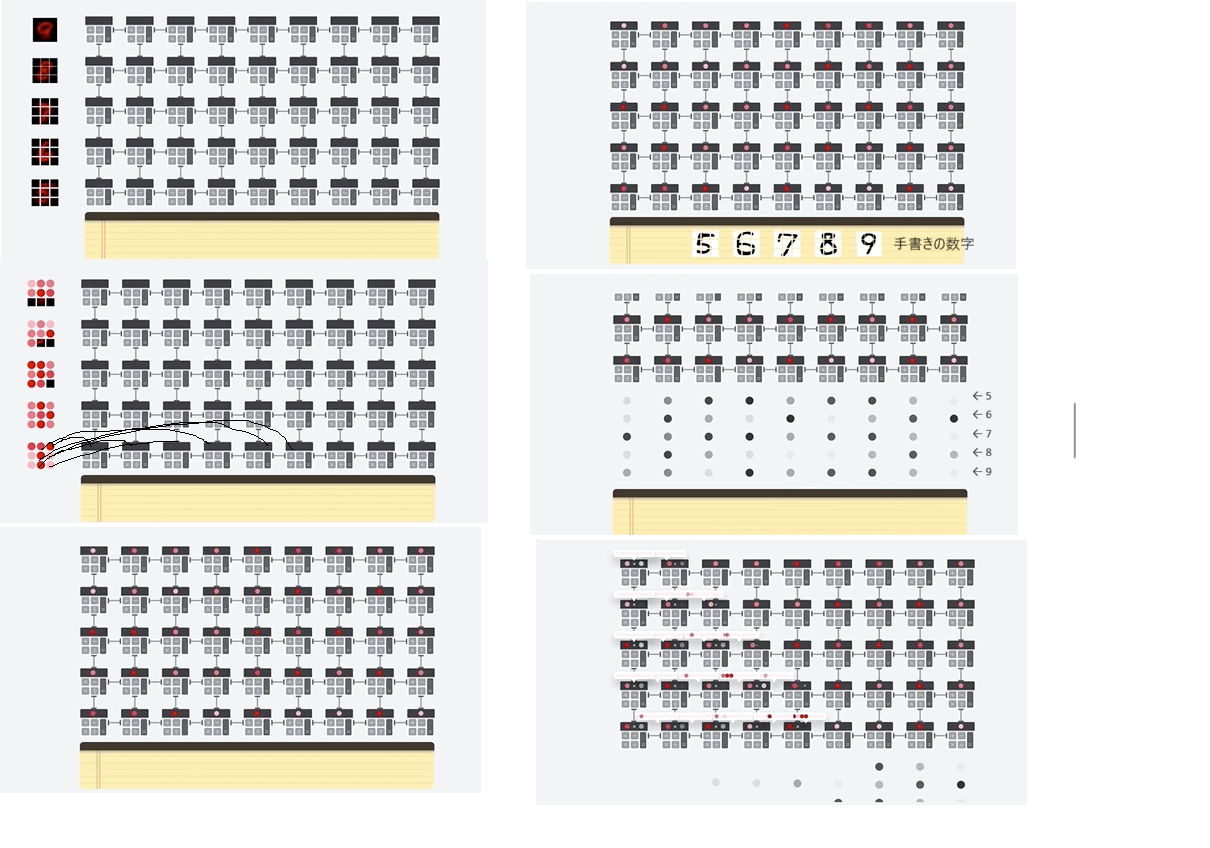
\includegraphics[width=15cm]{./capture/TPU.png}
  \caption{TPUでは、メモリからMatrix Multiplication Unit(MXU)にパラメータを読み込み(画像左列)、次にメモリからデータを読み込む(画像右列)。行列乗算演算中にメモリアクセスが無いため、高いスループットを達成できる。 (https://cloud.google.com/tpu/docs/intro-to-tpu?hl=ja 動画よりキャプチャ)}
  \label{fig:TPU}
\end{figure}



\subsubsection{量子化(Quantization)}
ネットワークが大きくなると、大量のパラメータをメモリで保持する必要があり、メモリの使用量が増加する。そのため、64bitの浮動小数点を32bitなどの下位の精度に変換することで、メモリの使用量を削減することができる。このような変換を量子化と呼ぶ。
\par
浮動小数点とは、指数部と仮数部に分かれている数値表現のことであり、64bitの浮動小数点は、指数部11bit、仮数部52bitで構成されている。一方、32bitの浮動小数点は、指数部8bit、仮数部23bitで構成されている (図\ref{fig:float32})。
機械学習用のbfloat16は、指数部8bit、仮数部7bitで構成されている。
\begin{figure}[htbp]
  \centering
  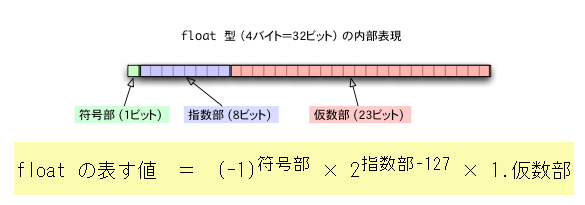
\includegraphics[width=15cm]{./capture/float32.png}
  \caption{32bit浮動小数点の内部表現 (https://www.cc.kyoto-su.ac.jp/~yamada/programming/float.html より引用)}
  \label{fig:float32}
\end{figure}

\par
例えば、64bitの浮動小数点を使った場合、パラメータが1024個だった時には、8byte×1024=8KB、1024×1024個だった時には、8MB、1024×1024×1024個だった時には、8GBのメモリが必要となる。一方、32bitの浮動小数点を使った場合、パラメータが1024個だった時には、4KB、1024×1024個だった時には、4MB、1024×1024×1024個だった時には、4GBのメモリが必要となる。
BERTでは、およそ0.6GBのメモリが必要となるが、量子化を行うことで、0.3GBのメモリで動作するようになる。
\par
ただし、浮動小数点の性質上、量子化を行うことで、精度が下がる。例えば、Yin et al.(2017) は図\ref{fig:32bitVS6bit}のように、量子化を行うことで、検出時間は1/4~1/5になり、精度が下がったり、余白が広くなっていることを示している。 
\begin{figure}[htbp]
  \centering
  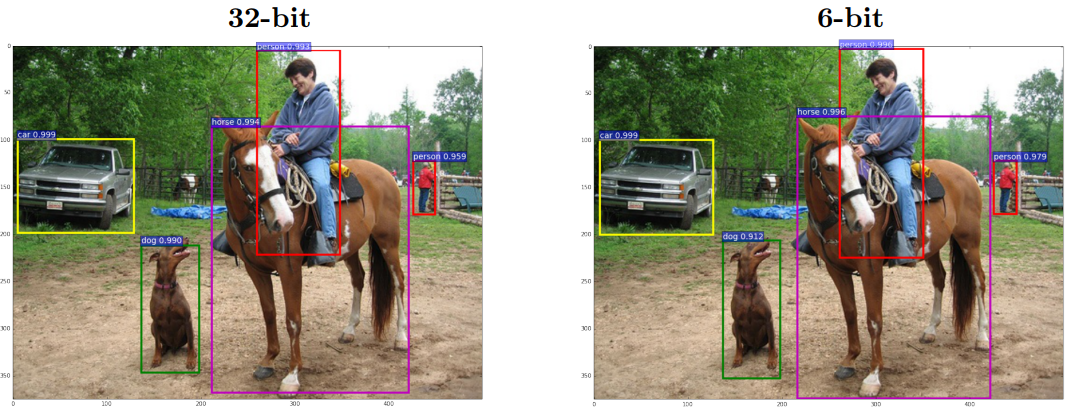
\includegraphics[width=15cm]{./capture/32bitVS6bit.png}
  \caption{量子化による精度の低下 (Yin et al.(2017) より引用): 6bitにしたときに、各分別結果の値が若干異なることがわかる。}
  \label{fig:32bitVS6bit}
\end{figure}

\subsection{蒸留}
蒸留とは、大きなモデル(教師モデル)の知識を小さなモデル(生徒モデル)に継承する手法である。蒸留では、教師モデルは学習済みとし重みを固定し、生徒モデルの重みを学習する。データを与えた時の教師モデルの出力をソフトマックス関数で確率分布に変換し、生徒モデルの出力との誤差を最小化するように学習を行う。少ない層でも高い精度の出力を行うことができる(図\ref{fig:distillation})。
\begin{figure}[htbp]
  \centering
  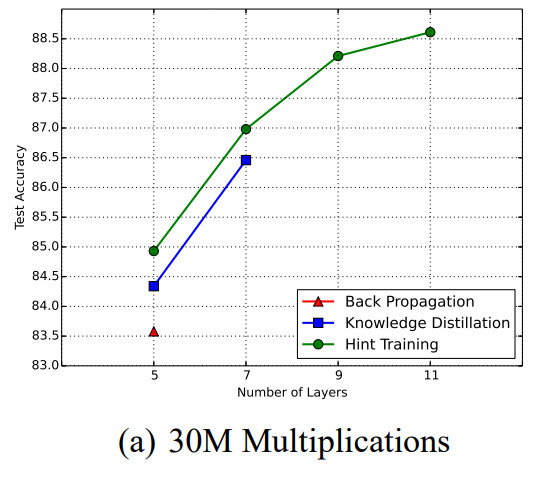
\includegraphics[width=10cm]{./capture/distillation.png}
  \caption{蒸留後の生徒モデルの層数(横軸)と精度(縦軸) (Romero et al.(2015) より引用)}
  \label{fig:distillation}
\end{figure}

\subsection{プルーニング}
プルーニングとは、モデルのパラメータを削減する手法である。プルーニングでは、学習後にモデルのパラメータのうち、重要でないパラメータを削除する。例えば、閾値を決めて、その閾値を超えるパラメータを削除する。プルーニングを行うことで、モデルのサイズを削減し、計算量を削減することができる(図\ref{fig:pruning})。
\begin{figure}[htbp]
  \centering
  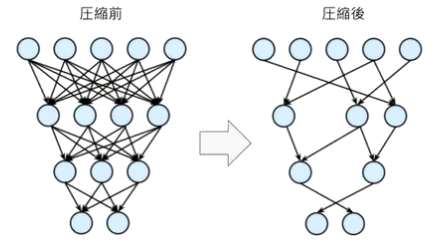
\includegraphics[width=10cm]{./capture/pruning.png}
  \caption{プルーニングのイメージ図}
  \label{fig:pruning}
\end{figure}

例えば、佐々木など(2015)は、全結合層のパラメータ削減手法を比較している。閾値パラメータ$\alpha$が最小の0.5の時にはすでにおよそ50\%のパラメータが削減されるが、精度は92\%からわずかに0.34\%下がるだけであることがわかっている(図\ref{fig:pruning_table})。
\begin{figure}[htbp]
  \centering
  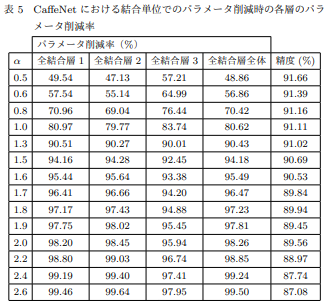
\includegraphics[width=10cm]{./capture/pruning_table.png}
  \caption{もともとのモデルの精度は92\%程度 (佐々木など(2015) より引用)}
  \label{fig:pruning_table}
\end{figure}

\clearpage

\section{応用技術}
\subsection{MobileNet : Efficient Convolutional Neural Networks for Mobile Vision Applications}
MobileNetsは、軽量な画像認識畳み込みニューラルネットワークである。
深層学習による画像分類予測は2017年でほとんどが完成されており、それ以降は軽量化、高速化、精度向上が求められてきた。MobileNetsは、そうした流れの中で開発された。
\par
まず、一般的な畳み込みレイヤーでは、入力$H \times W \times C$の画像に対して、$K \times K \times C$ のフィルタを$M$個適用して、$H \times W \times M$の出力を得る。このときの計算量は、$H \times W \times C \times K \times K \times M$である。
\par
MobileNetsでは、Depthwise Separatable ConvolutionとPointwise Convolutionという畳み込み手法を用いて、計算量を削減している。
\par
Depthwise Separatable Convolutionは、フィルタのチャンネル数が1で、チャンネルを通した畳み込みを行わず、チャンネルごとに畳み込みを行う手法である。この手法では、入力$H \times W \times C$の画像に対して、$K \times K \times 1$のフィルタを適用して、$H \times W \times C$の出力を得る。このときの計算量は、$H \times W \times C \times K \times K$となり、通常の畳み込みに比べて、$C$倍の計算量削減が可能である。
\par
Pointwise Convolutionは、GoogLeNetにも用いられた畳み込み手法で、$1 \times 1 \times C$のフィルタを$M$個適用して、チャンネル数を変換する手法である。この手法では、入力$H \times W \times C$の画像に対して、$1 \times 1 \times M$のフィルタを適用して、$H \times W \times M$の出力を得る。このときの計算量は、$H \times W \times C \times M$となり、通常の畳み込みに比べて、$K \times K$倍の計算量削減が可能である。
\par
通常の畳み込みに相当する部分を、Depthwise Separatable ConvolutionとPointwise Convolutionで担うことで、計算量は以下の削減される。
\begin{align}
  \text{通常の畳み込み} & : H \times W \times C \times K \times K \times M \\
  \text{MobileNets} & : H \times W \times C \times K \times K + H \times W \times C \times M
\end{align}

\subsection{DenseNet : Densely Connected Convolutional Networks}
DenseNetは、2016年に提案された画像認識畳み込みニューラルネットワークである。
特徴は、Dense Blockと呼ばれるブロックを用いて、畳み込み層間を結合する手法である。
Dense Block内は、複数の畳み込み層が結合されており、$l$番目の入力は、$l-1$番目までの出力を全て結合して入力とする。
\begin{align}
  x_l = H_l([x_0, x_1, \cdots, x_{l-1}])
\end{align}
ここで、$H_l$は、$l$番目の畳み込み層を表し、$[x_0, x_1, \cdots, x_{l-1}]$は、$l-1$番目までの出力を結合したものである。最初のチャンネル数が$k_0$で、出力が$k$チャンネルの場合、Block内の畳み込み層を経るごとに、出力は$k$チャンネル増加する。結果、Dense Blockの層数が$n$、フィルタ数が$k$の場合、Blockに$k_0$チャンネルの入力を与えると、$k_0 + k \times n$の出力が得られることとなる。
\par
こうして得られた出力は、Transition Layerと呼ばれる畳み込み層で、チャンネル数を削減する。Transition Layerは、Batch Normalization、畳み込み、プーリングの3つの層から構成されている。
\par
図\ref{fig:CNN_connection}では、通常の畳み込み、ResNet、DenseNetの結合方法の違いを示している。通常の畳み込みでは、$l$番目の畳み込み層の入力は、$l-1$番目の出力のみである。ResNetでは、$l$番目の畳み込み層の入力は、$l-1$番目の出力と$l-2$番目の出力を結合して入力とする。DenseNetでは、$l$番目の畳み込み層の入力は、$l-1$番目までの出力を全て結合して入力とする。

\begin{figure}[htbp]
  \centering
  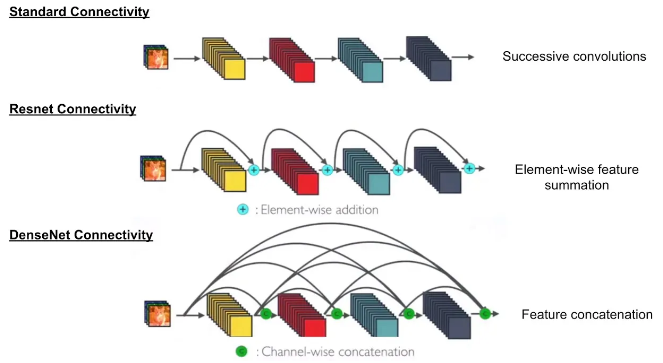
\includegraphics[width=10cm]{./capture/CNN_connection.png}
  \caption{畳み込み層間の結合方法 : (上)通常の畳み込み, (中)ResNetの結合方法, (下)DenseNetの結合方法 (https://cvinvolution.medium.com/why-isnt-densenet-adopted-as-extensive-as-resnet-1bee84101160 より引用)}
  \label{fig:CNN_connection}
\end{figure}

\subsection{Batch Normalization, Layer Normalization, Instance Normalization}
Batch Normalization, Layer Normalization, Instance Normalizationは、ニューラルネットワークの正則化手法である。
\par
Batch Normalizationは、ミニバッチに含まれるサンプルの同一チャンネルが同一分布に従うように正規化する。効果がミニバッチの数に依存し、ミニバッチの数が少ないと効果が低下する。
\par
Layer Normalizationは、それぞれのサンプルのすべてのピクセルが同一分布に従うように正規化する。ミニバッチの数に依存しないため、ミニバッチの数が少なくても効果がある。
Instance Normalizationは、それぞれのサンプルの、同一チャンネルのすべてのピクセルが同一分布に従うように正規化する。コントラストの強調や色調・テクスチャの変換に使われることが多い。
\begin{figure}[htbp]
  \centering
  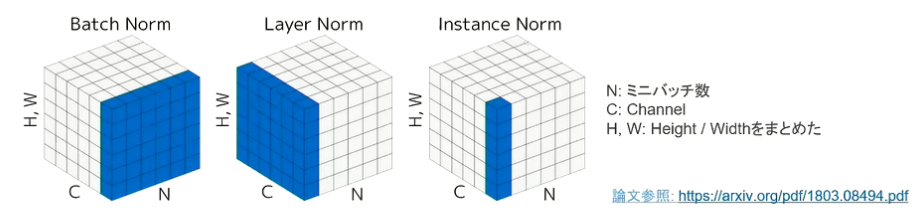
\includegraphics[width=15cm]{./capture/Batch_Layer_Instance_Norm.png}
  \caption{Batch Normalization, Layer Normalization, Instance Normalizationの比較 (https://arxiv.org/pdf/1803.08494.pdf より引用)}
\end{figure}

\subsection{WaveNet : A Generative Model for Raw Audio}
WaveNetは、2016年に提案された音声生成モデルである。
\begin{figure}[htbp]
  \centering
  \begin{subfigure}[b]{0.45\textwidth}
    \centering
    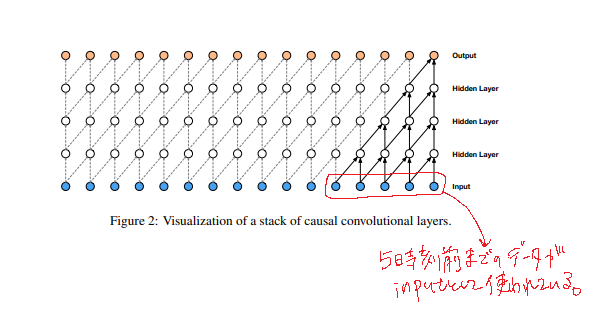
\includegraphics[width=\textwidth]{./capture/WaveNet_1.png}
    \caption{既存の畳み込み}
    \label{fig:WaveNet_1}
  \end{subfigure}
  \hfill
  \begin{subfigure}[b]{0.45\textwidth}
    \centering
    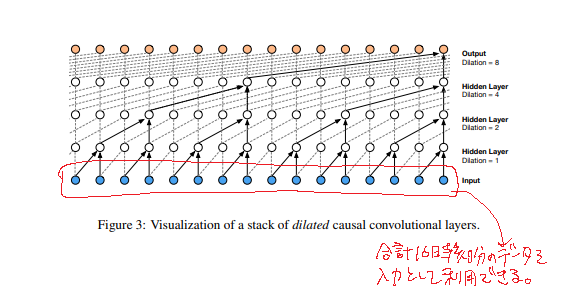
\includegraphics[width=\textwidth]{./capture/WaveNet_2.png}
    \caption{Dilatad Convolution}
    \label{fig:WaveNet_2}
  \end{subfigure}
  \caption{WaveNetの畳み込み手法 : (左)既存の畳み込み, (右)Dilatad Convolution(飛ばし飛ばしで畳み込むことでより多くの受容野を入力とできる特徴がある) (https://arxiv.org/pdf/1609.03499.pdf より引用)}
\end{figure}
WaveNetは、Dilatad Convolutionを用いて、音声の生成を行う。Dilatad Convolutionは、飛ばし飛ばしで畳み込むことで、より多くの受容野を入力とできる特徴がある。図\ref{fig:WaveNet_1}では、既存の畳み込みの受容野は、5つのピクセルであるが、Dilatad Convolutionを用いることで、受容野を16つのピクセルに拡張することができる(図\ref{fig:WaveNet_2})。

\clearpage
\paragraph{参考文献}
\begin{enumerate}
  \item 岡谷貴之/深層学習 改訂第2版 [機械学習プロフェッショナルシリーズ]/ 講談社サイエンティフィク/ 2022-01-17
  \item 深層学習とゲーム理論 \url{https://www.slideshare.net/slideshow/marl/234128570#6}
  \item 強化学習 星の本棚/ \url{https://yagami12.hatenablog.com/entry/2019/02/22/210608} 2024年6月21日閲覧
  \item 分散深層学習とモデル並列性 Preferred Networks \url{https://tech.preferred.jp/ja/blog/model-parallelism-in-dnn}
  \item Cloud TPU の概要 Google Cloud \url{https://cloud.google.com/tpu/docs/intro-to-tpu?hl=ja}
  \item 浮動小数点数型と誤差 京都産業大学\url{https://www.cc.kyoto-su.ac.jp/~yamada/programming/float.html}
  \item Quantization and Training of Low Bit-Width Convolutional Neural Networks for Object Detection (Yin et al.(2016) \url{https://arxiv.org/abs/1612.06052})
  \item ニューラルネットワークの全結合層におけるパラメータ削減手法の比較 佐々木など(2015){https://db-event.jpn.org/deim2017/papers/62.pdf}
  \item Why isn’t DenseNet adopted as extensive as ResNet? \url{https://cvinvolution.medium.com/why-isnt-densenet-adopted-as-extensive-as-resnet-1bee84101160}
  \item Group Normalization (Wu and He(2018)) \url{https://arxiv.org/pdf/1803.08494.pdf}
  \item WAVENET: A GENERATIVE MODEL FOR RAW AUDI (Oord et al.(2016)) \url{https://arxiv.org/pdf/1609.03499.pdf}
\end{enumerate}

\newpage
\end{document}